\section{Environment}

The measurements are captured on the \code{gp1} system provided by Faculty of Nuclear Sciences and Physical Engineering, Czech Technical University with following specifications \ref{table:env-gp1}:

\begin{table}[H]
  \centering
  \begin{tabular}{ | l | l | }
    \hline
    CPU             & Intel Xeon CPU E5-2630 v3 (2.40\,GHz)    \\
    \hline
    GPU             & NVIDIA Quadro P6000 (24\,GB, CUDA 6.1)   \\
    \hline
    RAM             & 128\,GB                                  \\
    \hline
    Driver          & 465.31                                   \\
    \hline
    OS              & Arch Linux (kernel 4.12.9, KPTI enabled) \\
    \hline
    Host compiler   & GCC g++ 11.1.0                           \\
    \hline
    Device compiler & nvcc v11.3.58                            \\
    \hline
  \end{tabular}
  \caption{Hardware and software specification of the \code{gp1} system.}
  \label{table:env-gp1}
\end{table}

Furthermore, the optimization flag is set to \code{-O3}. \CC\,dialect is set to \CC17 when benchmarking against different implementations, although \CC14 is supported as well.

\section{Testing methodology}

As the execution of code on the device is not deterministic, it is hard to prove the complete absence of errors and bugs of the solution. Nevertheless, for each of the B-Tree implementations, a set of unit tests is prepared. This unit test suite rigorously examines if each operation preserves the valid tree state, which has proved to be helpful when optimizing the performance of the tree without sacrificing correctness. \code{GoogleTest} framework \cite{gtest} is the framework of choice used for writing these unit test suites.

For the host implementation, unit tests do include assertions of the internal states of a node to aid the development and catch bugs early on. On the device side, though, asserts on the device code are limited, and unit tests make their assertions only on the result after operation completion, as \code{GoogleTest} is unfortunately not supported on the device code.

Even though \code{cuda-gdb} does work on GPU-specific code, debugging of a kernel is a pain-staking process. Pinpointing race conditions can be difficult, especially without any prior context, and any potential issues might arise only when dealing with a large number of items in B-Tree. To better understand the behavior of GPU B-Tree operations and help find concurrency issues easier, a complimentary web-based visual debugger has been developed in React, seen in Figure \ref{figure:debugger}.

Macro functions have been inserted through the implementations, which are enabled by defining \code{DEBUGGER} in the source code. With this flag, the implementation will emit debugging commands into the standard output, which can be inserted into the web app.

\begin{figure}
  \centering
  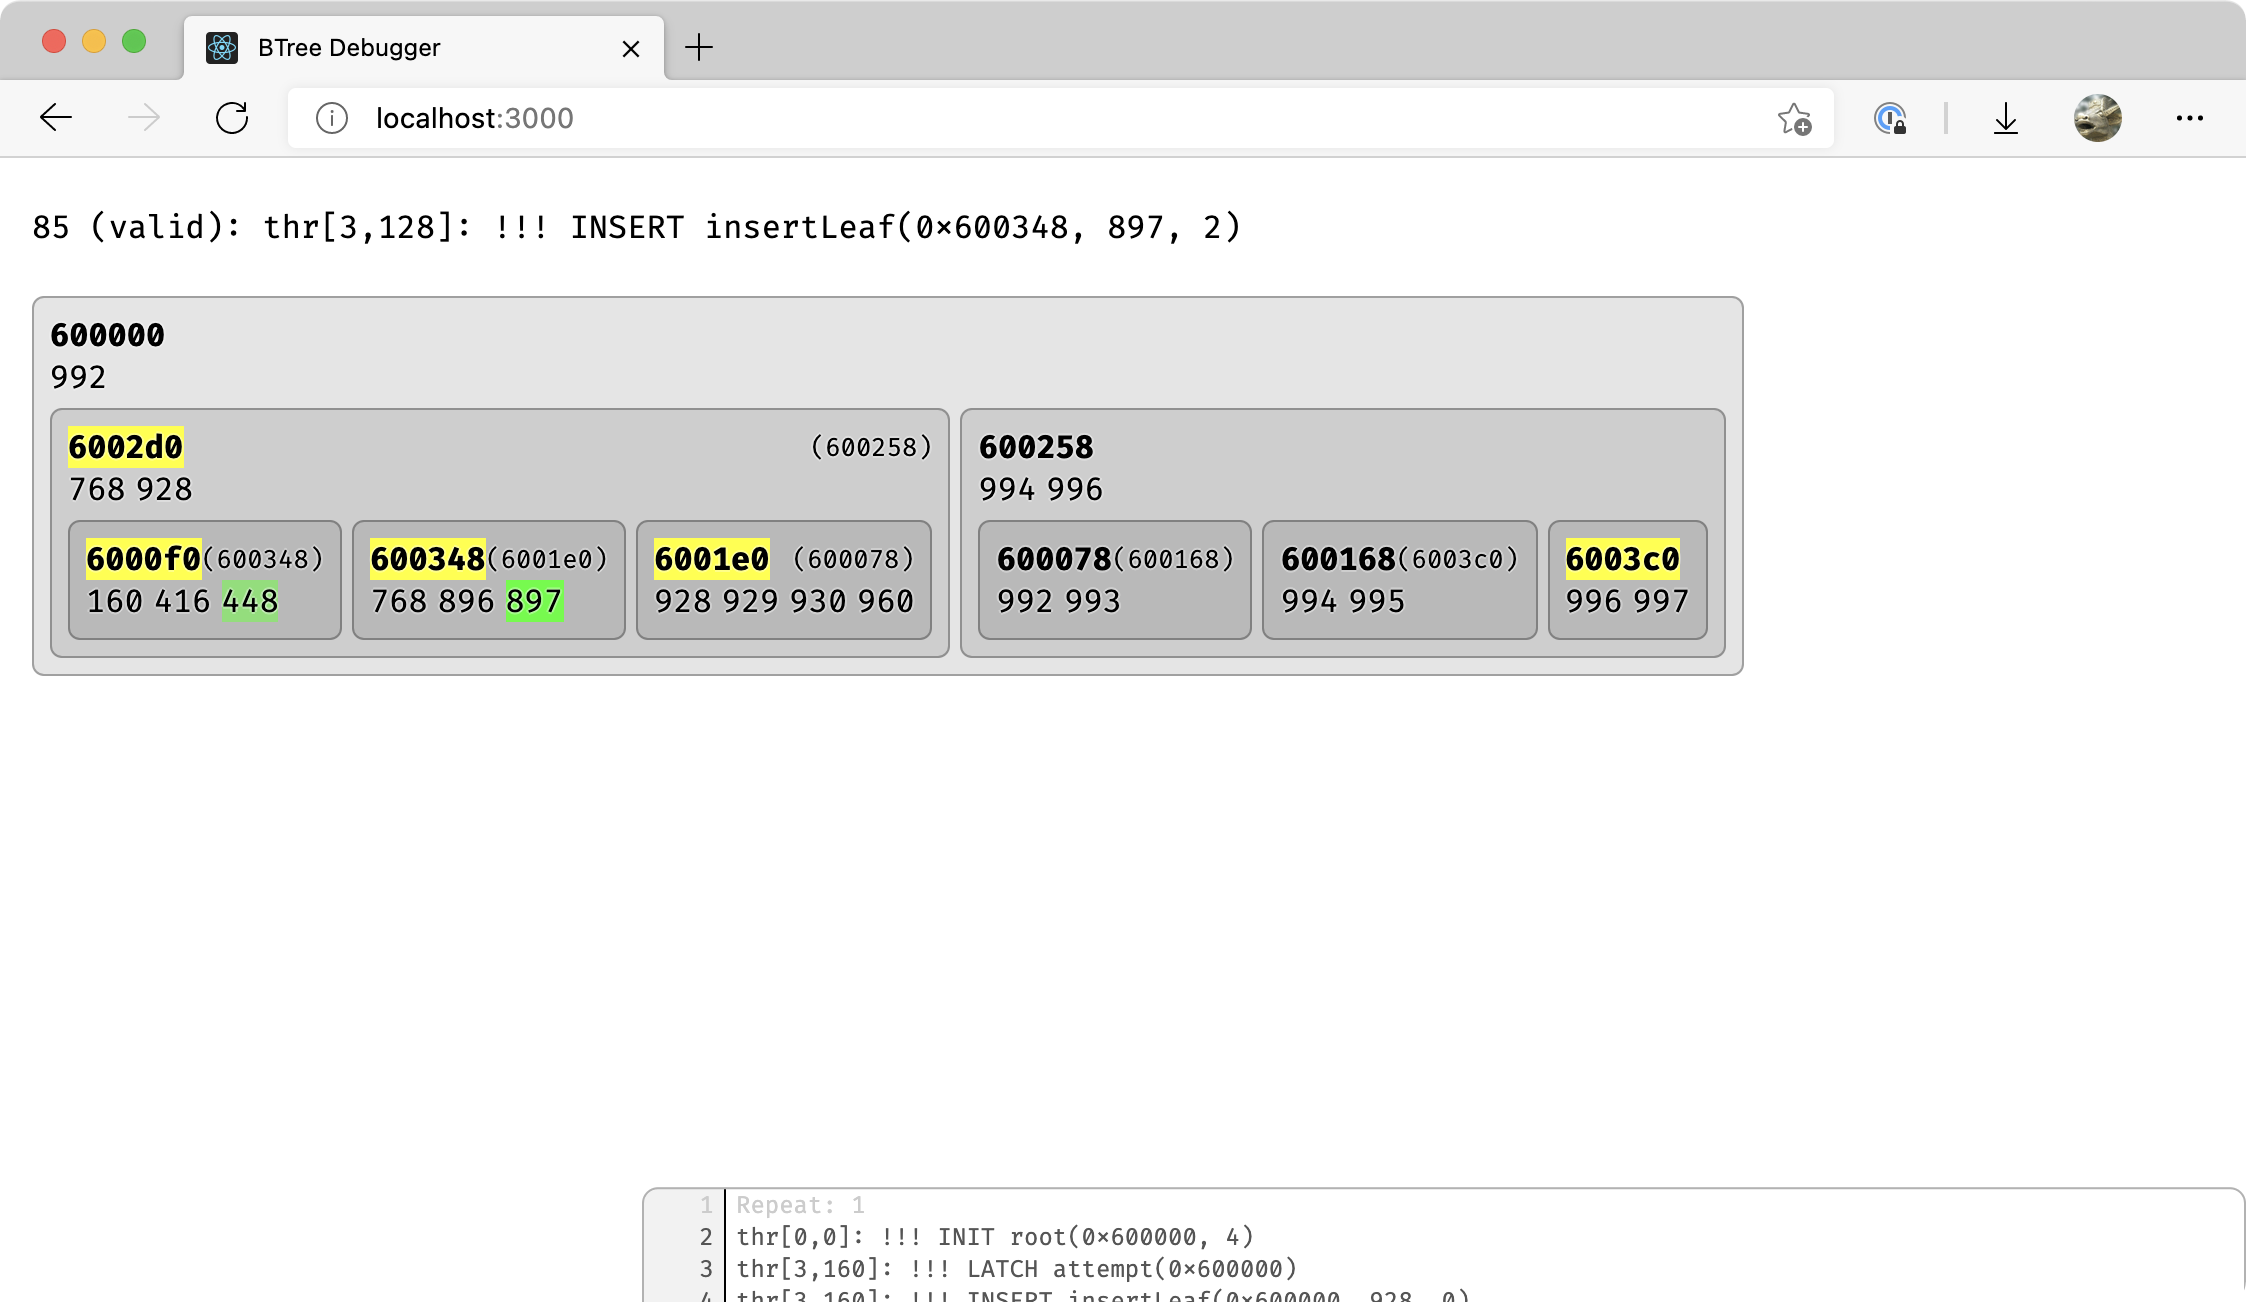
\includegraphics[width=\textwidth]{components/figure/debugger.png}
  \caption{Web based visual debugger displaying the internal state of a tree. Red boxes denote split nodes not yet inserted to the parent node. Yellow-highlighted node addresses indicate that a thread has latched that node.}
  \label{figure:debugger}
\end{figure}

In the case of multiple B-Tree variants, to avoid duplicating tests and ensure the correctness of both implementations, typed tests are used to repeat the same logic over a list of types \cite{gtest-advanced}, as seen in Listing \ref{lst:gtest-typed}. The \code{typename} of each class will be available as a static field within \code{TestFixture} itself.

\begin{listing}
  \begin{minted}{cpp}
template <typename C> class TestSuite : public testing::Test {
public:
  using Implementation = C;
};

using TypeList = ::testing::Types<A, B>;
TYPED_TEST_SUITE(TestSuite, TypeList);

TYPED_TEST(TestSuite, Test) {
  typename TestFixture::Implementation impl;
  // ... rest of test implementation
}
    \end{minted}
  \caption{Snippet of a \code{GoogleTest} typed test}\label{lst:gtest-typed}
\end{listing}

\section{Benchmarking methodology}

After measuring execution times from chosen implementations, we calculate the speedup as the ratio of serial execution time on the CPU and parallel execution time on the GPU.

$$\mathit{Speedup} = \frac{\tau_{\mathit{CPU}}}{\tau_{\mathit{GPU}}}$$

\section{Numerical network microbenchmark}

\todo{Add numerical mesh microbenchmark - numerical networks}


To determine the performance speedup between the GPU and the CPU implementation, a micro-benchmark is introduced with a simple use case. The benchmark consists of incremental inserting and querying unstructured numerical cube mesh.

\section{Comparison against known implementations}

This section describes the comparison of the thesis implementation against other GPU and CPU based implementations. \todo{add cites}

For all of the experiments, 32-bit keys and values are used. Different kinds of pair sequences were used as the input data and each implementation is executed and measured 10 times. Results presented here are averaged. Measurement of CPU based variants are measured using {std::chrono::high\_resolution\_clock::now}, whereas the GPU based ones are measured using CUDA runtime API. The time spent on copying the data from host to device is not included in the measurement.

\todo{Add search benchmark}

\todo{Add insertion benchmark}

\todo{Add an explanation why \cite{awad} is 2-3 times faster than our implementation.} Improved memory access